\chapter{Исследовательская часть}

В данном разделе будет приведен пример работы программы, а также проведен сравнительный анализ алгоритма поиска для сбалансированного и несбалансированного бинарного дерева поиска.

\section{Демонстрация работы программы}

На рисунке~\ref{img:example}  представлен пример работы программы для поиска в сбалансированном бинарном дереве поиска.
Осуществляется выбор типа дерева поиска, в него происходит добавление элементов, после чего в нём проводится поиск числа.

\begin{figure}[h]
	\centering
	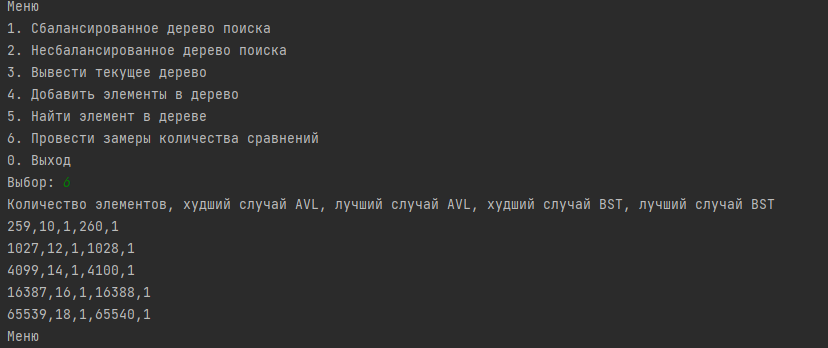
\includegraphics[width=1.0\textwidth]{img/example.png}
	\caption{Пример работы программы}
	\label{img:example}
\end{figure}

\section{Замеры времени и количества сравнений}

Были произведены замеры времени нахождения числа в дереве в худшем и лучшем случае.

Результаты замеров в секундах представлены в таблице \ref*{tbl:times}.

\begin{table}[h]
	\begin{center}
		\begin{threeparttable}
			\captionsetup{justification=raggedright,singlelinecheck=off}
			\caption{Результаты временных замеров}
			\label{tbl:times}
			\begin{tabular}{|r|r|r|r|r|}
				\hline
				Элементы & Худший AVL & Лучший AVL & Худший BST & Лучший BST \\
				\hline
				259 & 0.0011 & 0.0001 & 0.0034 & 0.0001 \\ 
				\hline
				1027 & 0.0026 & 0.0001 & 0.0434 & 0.0001 \\ 
				\hline
				4899 & 0.0039 & 0.0001 & 0.7493 & 0.0001 \\ 
				\hline
				16387 & 0.0075 & 0.0001 & 5.1382 & 0.0001 \\ 
				\hline
				65539 & 0.0124 & 0.0001 & 53.3482 & 0.0001 \\ 
				\hline
			\end{tabular}
		\end{threeparttable}
	\end{center}
\end{table}

\newpage
Были произведены замеры необходимого количества сравнений для нахождения числа в дереве в худшем и лучшем случае.

Результаты замеров представлены в таблице \ref*{tbl:time}.

\begin{table}[h]
	\begin{center}
		\begin{threeparttable}
			\captionsetup{justification=raggedright,singlelinecheck=off}
			\caption{Результаты замеров количества сравнений}
			\label{tbl:time}
			\begin{tabular}{|r|r|r|r|r|}
				\hline
				Элементы & Худший AVL & Лучший AVL & Худший BST & Лучший BST \\
				\hline
				259 & 10 & 1 & 260 & 1 \\ 
				\hline
				1027 & 12 & 1 & 1028 & 1 \\ 
				\hline
				4899 & 14 & 1 & 4100 & 1 \\ 
				\hline
				16387 & 14 & 1 & 16388 & 1 \\ 
				\hline
				65539 & 16 & 1 & 65540 & 1 \\ 
				\hline
			\end{tabular}
		\end{threeparttable}
	\end{center}
\end{table}
По таблице \ref*{tbl:time} были построены рисунки \ref*{fig:avl-res} -- \ref*{fig:bst-res}, на них можно увидеть зависимость количества сравнений при поиске в худшем случае для АВЛ-дерева и бинарного дерева поиска.

\begin{figure}[h]
	\centering
	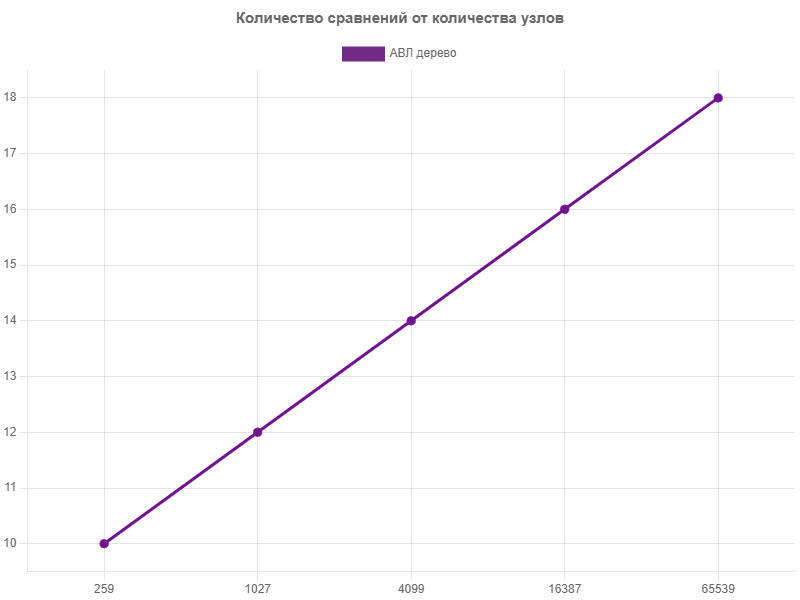
\includegraphics[height=0.4\textheight]{img/avl-graph.png}
	\caption{Результаты замеров количества сравнений в худшем случае при поиске в АВЛ-дереве}
	\label{fig:avl-res}
\end{figure}

\begin{figure}[h]
	\centering
	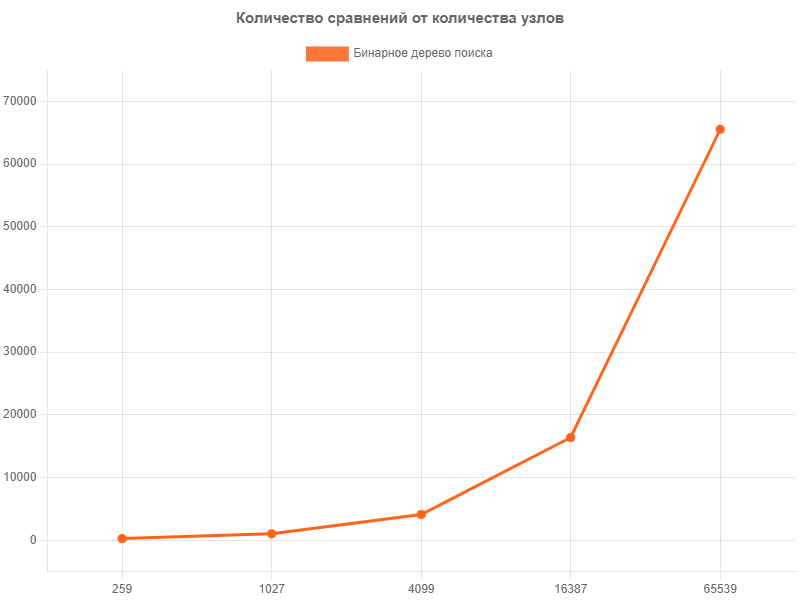
\includegraphics[height=0.4\textheight]{img/bst-graph.png}
	\caption{Результаты замеров количества сравнений в худшем случае при поиске в несбалансированном бинарном дереве поиска}
	\label{fig:bst-res}
\end{figure}

\newpage


По полученным данным можно увидеть, что количество сравнений при поиске в АВЛ-дереве действительно логарифмически зависит от количества узлов, в то время как для БДП зависимость линейная.

\newpage
\section*{Вывод}

В результате эксперимента было получено, что в лучшем случае количество сравнений для АВЛ-дерева и несбалансированного бинарного дерева поиска одинаково и равно 1 для любого рассмотренного количества узлов.
В худшем случае количество сравнений в АВЛ-дереве более чем в 1000 раз меньше, чем в несбалансированном бинарном дереве поиска при количестве узлов большем или равном 16388.